% ================================ LE MODALITÀ DI AES ===================================

\chapter{Le modalità di AES}

%TODO: ECB, CBC, CTR, GCM, CBC-MAC, CFB, OCB, XTS, OFB
%TODO: Section sulle MAC
%TODO: Section Authenticated encryption
%TODO: Consigli generali? Non riusare mai lo stesso IV (spiegare cos'è la IV) e rendere l'IV non predicibile!
%TODO: spiegare cos'è il nonce (cercare traduzione in italiano).
%TODO: IV vs nonce.

%TODO: aggiungere delle immagini se possibile.

%TODO: Aggiungere i vari tipi di padding? Prima o dopo la spiegazione delle modalità? Prima direi, dopo l'iv, nonce, ecc.

%TODO: Magari approfondire le modalità che andrò a implementare.

%TODO: 0-Padding, 1-0-Padding, ISO, ...

% =======================================================================================

% ---------------------------- SECTION: INTRODUZIONE ------------------------------------

%TODO: In questo capitolo/In questa parte tratteremo le varie modalità di crittografia disponibili su/per AES. Queste ci permetteranno di cifrare messaggi di varia lunghezza.

\section{Introduzione}

% ---------------------------- SECTION: PERCHÉ SERVE UNA/LE MODALITÀ? PERCHÉ USARE UNA/LE MODALITÀ? A COSA SERVONO LE MODALITÀ? ------------

\section{A cosa servono le modalità?} %TODO: A cosa servono le modalità? oppure Perché usare le modalità

%TODO: Le modalità sono necessarie, perché AES è un cifrario a blocchi, prende in input un blocco e una chiave di 16 bytes

%TODO: Le modalità servono, perché AES è un cifrario a blocchi di 16 bytes, dopo aver preso un blocco e una chiave in input restituisce un altro blocco della medesima grandezza/lunghezza.

%TODO: Quindi, se si desidera/vuole cifrare una sequenza di bytes di lunghezza/grandezza maggiore di 16 bytes, bisogna/è necessario utilizzare una \emph{modalità di operazione} o \emph{modalità di cifratura}.

%TODO: Queste modalità sono indipendenti dal tipo di cifrario sottostante/che sta alla base.

\textsf{\small }

\begin{comment} %TODO: uncomment or remove?
\begin{figure}[H]
	\centering
	\includegraphics[width=.9\textwidth, height=.9\textheight, keepaspectratio]{./images/aes_modes/aes_modes.png}
	\caption{Modalità di AES}
	\label{fig:aes_modes}
\end{figure}
\end{comment}

% -------------------------- SECTION: IV, NONCE, SALT E PEPPER --------------------------

\section{IV, Nonce, Salt e Pepper} %TODO: IV, Nonce, Sale e Pepe?

%TODO: Prima di poter trattare le modalità è necessario introdurre alcuni componenti/elementi che ci serviranno (nella creazione ...). (Questi sono l'IV, il nonce, il sale e il pepe).

\textsf{\small }

\subsection{Nonce | Number Used Once} %TODO: oppure solo Nonce

%TODO: Aggiungere dove viene usato.

%TODO: Il nonce, \emph{\textbf{n}umber used \textbf{once}} (numero utilizzato una volta), sono dei bits (ovvero un numero) che vengono utilizzati una singola volta. Il riutilizzo non è proibito, ma deve essere limitato.

%TODO: Viene utilizzato nei protocolli di autenticazione per garantire la sicurezza nelle comunicazioni (private) (ed evitare replay attacks [da spiegare in un altro capitolo (e aggiungere la \ref alla pagina volendo)]).

\textsf{\small }

\begin{figure}[H]
	\centering
	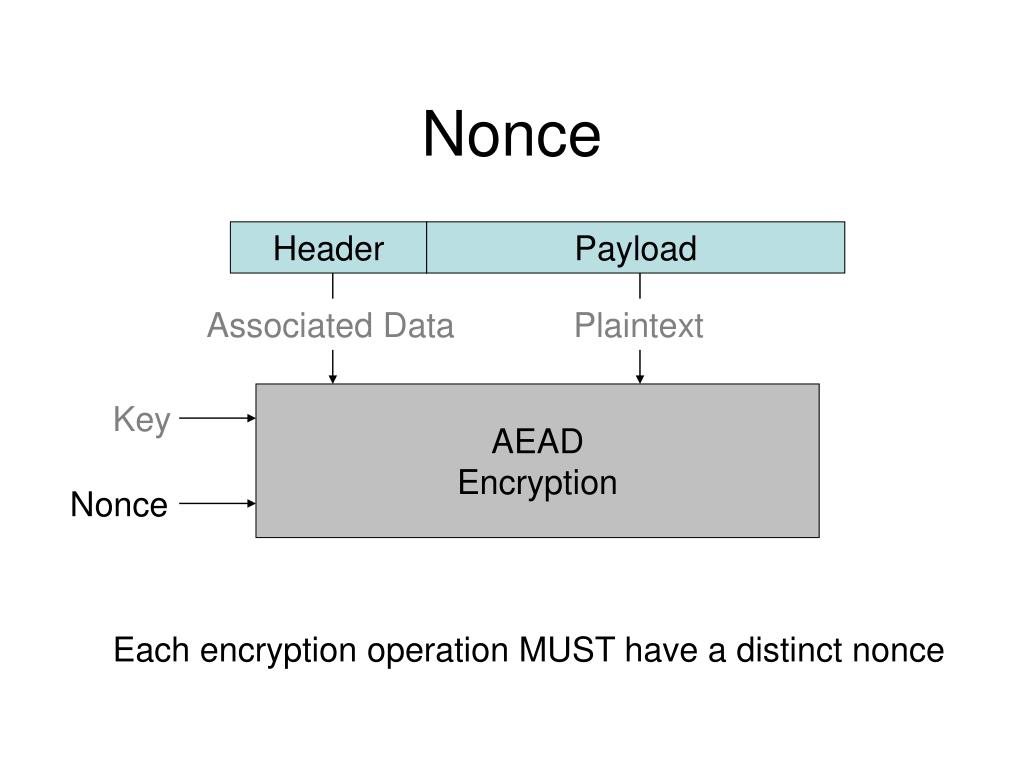
\includegraphics[width=.9\textwidth, height=.9\textheight, keepaspectratio]{./images/iv_nonce_salt_pepper/nonce.png}
	\caption{Nonce}
	\label{fig:nonce}
\end{figure}

\subsubsection{Nonce sequenziali}

%TODO: Prevenisco/Garantiscono la non ripetizione, se molto grandi.

\textsf{\small }

%TODO: subsubsection Nonce random?

\subsection{IV | Initialization Vector} %TODO: Oppure solo IV; prima era L'IV; Initialization Vector | IV

%TODO: L'initialization vector o anche definito/chiamato starting variables è un input di dimensione fissa, ovvero un numero arbitrario che viene fornito/adoperato per impostare lo stato iniziale di un algoritmo crittografico. Viene utilizzato in varie modalità di cifratura per randomizzare la cifratura in modo da produrre/generare diversi testi cifrati anche se lo stesso testo viene cifrato molteplici volte.

%TODO: È simile al nonce, ma deve essere casuale/random. Quindi i nonce sequenziali non andrebbero bene.

%TODO: È prioritario/molto importante che l'IV sia:
%TODO: itemize: impredicibile
%TODO: sempre diverso, mai riutilizzare lo stesso/un IV!

\textsf{\small }

\subsection{IV vs Nonce} %TODO: forse questa non serve.

\textsf{\small }

\subsection{Salt} %TODO: Oppure Sale; Oppure Salt | Password Salting

%TODO: Il salt/sale/password salting viene utilizzato nelle password per incrementarne la sicurezza. Vengono aggiunti dei caratteri unici casuali alla password, in questo modo un attaccante non necessita solamente di un dizionario di password comuni, ma anche di uno per ogni tipo di sale possibile.

%TODO: Questo processo/tecnica è molto importante e viene utilizzata nei database affinché le password degli utenti siano sicure. (e non possano essere rubate).
%TODO: Le password non vengono mai, possibilmente, memorizzate nei database in chiaro, ma gli viene aggiunto il salt e poi viene eseguito l'hashing su esse.

\textsf{\small }

\begin{comment} %TODO: uncomment or remove?
\begin{figure}[H]
	\centering
	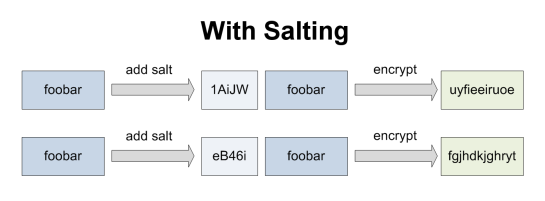
\includegraphics[width=1\textwidth, height=1\textheight, keepaspectratio]{./images/iv_nonce_salt_pepper/withsalting.png}
	\caption{Salt}
	\label{fig:salt}
\end{figure}
\end{comment}

\subsection{Pepper} %TODO: Oppure Pepe

%TODO: Il pepper/pepe è simile al salt/sale, ma questo a differenza del sale che è appena/meramente unico più che segreto, è un (singolo) carattere segreto appeso/aggiunto alla fine della password.

%TODO: Questo, (a differenza del sale) non viene memorizzato nello stesso database assieme alla password hash e al sale, ma a parte.

\textsf{\small }

%TODO: subsection: IV, Nonce, Salt, Pepper o magari salt e pepper non servono.

%TODO: subsection IV vs Nonce

% ---------------------------- SECTION: IL PADDING --------------------------------------

\section{Il padding}

\textsf{\small Un altro elemento utilizzato nei cifrari a blocchi è il padding. }
\textsf{\small Il padding serve per riempire i blocchi del cifrario con dei bytes.}

\textsf{\small È un modo per cifrare messaggi anche di grandezze che il cifrario non sarebbe in grado di decifrare.}
\textsf{\small Non aumenta la sicurezza, anzi se mal implementato può portare ad attacchi di padding (\emph{padding oracle attack}).} %TODO: portare/causare. %TODO: approfondire magari anche con \ref nel capitolo sugli attacchi.

\textsf{\small Grazie a questa tecnica, è possibile aggiungere, all'inizio, al centro o in fondo al messaggio, del nonsense per oscurare parti del messaggio che altrimenti sarebbero prevedibili, come: \emph{Caro...}, \emph{Gentile...}, \emph{Cordiali Saluti..}, ecc.}

\textsf{\small I principali meccanismi di padding sono: }

\begin{comment} %TODO: uncomment, magari mostrare degli esempi per ognuno di questi?
\begin{itemize}
	\item \textsf{\small \textbf{No padding}: }
	\item \textsf{\small \textbf{0-Padding}: Vengono aggiunti dei bytes con degli zeri alla fine dell'ultimo blocco, finché non abbiamo il corretto numero di bytes (in AES è 16 bytes); se già abbiamo il numero necessario di bytes, allora non viene aggiunto nulla}
	\item \textsf{\small \textbf{1-0-Padding}: Viene aggiunto un byte a 1 e il restante viene riempito da bytes di 0 finché non abbiamo il numero necessario di bytes; se il numero di bytes necessario è già presente, allora aggiungiamo un altro blocco.}
	\item \textsf{\small \textbf{ANSI X9.23 Padding}: Aggiungiamo bytes di 0 alla fine dell'ultimo blocco, finché non abbiamo 16 - 1 bytes. Nell'ultimo blocco inseriamo il numero totale di bytes a 0 che abbiamo aggiunto; se l'ultimo blocco è già pieno (corrisponde a 16 bytes), allora aggiungiamo blocco addizionale.}
	\item \textsf{\small \textbf{ISO 10126 Padding}: Vengono aggiunti dei bytes casuali in fondo all'ultimo blocco, finché non abbiamo 16 - 1 bytes e nell'ultimo byte inseriamo il numero totale di bytes casuali che abbiamo immesso; Se l'ultimo blocco è già 16 bytes, allora aggiungiamo un altro blocco.}
	\item \textsf{\small \textbf{PKCS#7}: Aggiungiamo il numero totale di bytes che restano per riempire il blocco in ogni byte rimanente, finché non abbiamo 16 bytes.}
	\item \textsf{\small }
	\item \textsf{\small }
\end{itemize}
\end{comment}

\begin{comment} %TODO: uncomment e approfondire.
\begin{itemize}
	\item \textsf{\small CMS (\emph{\textbf{C}ryptographic \textbf{M}essage \textbf{S}yntax}): }
	\item \textsf{\small PKCS#5: bytes di padding = 8 - numberOfBytes(clearText) mod 8}
	\item \textsf{\small PKCS#7: }
	\item \textsf{\small Bit: composto da 0x80 seguito da bytes di zeri.}
	\item \textsf{\small Zero length: questo padding è composto da zeri tranne per l'ultimo byte che è uguale al numero di bytes di padding.}
	\item \textsf{\small Null: il padding è composto da caratteri NULL.}
	\item \textsf{\small Space: il padding è composto da spazi bianchi.}
	\item \textsf{\small Random: padding formato da bytes casuali tranne per l'ultimo byte che è uguale al numero di bytes di padding.}
\end{itemize}
\end{comment}

% ---------------------------- SECTION: LE MODALITÀ -------------------------------------

\section{Le modalità} %TODO: oppure trovare un altro titolo: Panoramica sulle modalità? però l'ho già usato come titolo "panoramica".

%TODO: Qui, di seguito elencherò le caratteristiche e proprietà delle principali modalità di cifratura:

\textsf{\small }

%TODO: encryption vs message integrity
%TODO: volendo anche il MAC qui e poi anche dopo
%TODO: MAC, meccanismo a tre componenti: Secret Key, MAC Signing Algorithm, MAC Validation Algorithm.

\subsection{Modalità di cifratura senza integrità del messaggio}

%TODO: Queste modalità forniscono la cifratura del messaggio, ma non garantisco l'integrità del messaggio, ovvero/quindi non è assicurato che il messaggio non sia stato manomesso/alterato e quindi non è possibile accertare l'autenticazione del messaggio originale. %TODO: magari riguardare la parte dell'"accertare l'autenticazione del messaggio originale".

\begin{figure}[H]
	\centering
	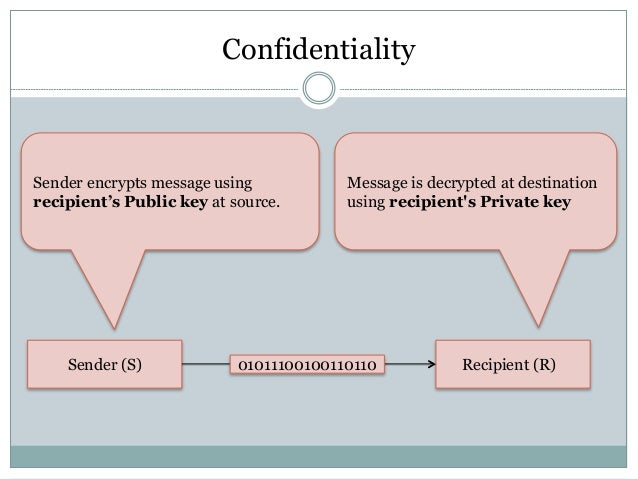
\includegraphics[width=.9\textwidth, height=.9\textheight, keepaspectratio]{./images/aes_modes/confidentiality.png}
	\caption{Confidenzialità}
	\label{fig:confidentiality}
\end{figure}

\textsf{\small }

\subsubsection{ECB | Electronic Code Book}

%TODO: Questa modalità di cifratura divide il nostro messaggio in diversi blocchi e ognuno di questi viene cifrato separatamente.

%TODO: Questa modalità manca il principio di diffusione (aggiungere \ref) e quindi cifra lo stesso messaggio nello stesso testo cifrato, quindi non vela (il pattern) dei dati/i dati.

%TODO: Quindi, se si encripta/cifra più di un blocco con la stessa chiave, non andrebbe usato.
%TODO: In generale, ECB è considerata una modalità obsoleta, da non utilizzare. È una modalità molto debole e poco sicura.

\textsf{\small }

\begin{figure}[H]
	\centering
	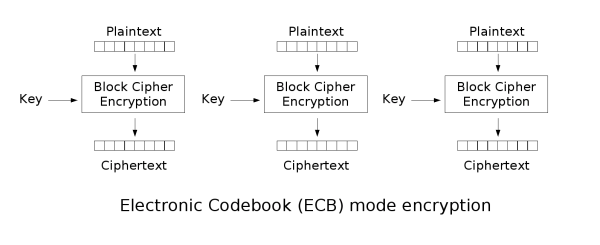
\includegraphics[width=.9\textwidth, height=.9\textheight, keepaspectratio]{./images/aes_modes/ecb_encryption.png} % mettere 1 e 1?
	\caption{ECB}
	\label{fig:ecb}
\end{figure}

\textsf{\small } %TODO: Come si deduce dall'immagine, ogni blocco viene cifrato indipendentemente. Viene inserito il messaggio in chiaro e la chiave all'interno del cifrario per ottenere il testo cifrato. Blocchi di testo in chiaro uguali vengono cifrato allo stesso modo.

%TODO: Per questo, osservando il testo cifrato è possibile riconoscere, se presenti nel testo in chiaro, parti cifrate allo stesso modo. 

%TODO: Per decifrare, eseguiamo l'operazione inversa, immettendo un blocco cifrato assieme alla chiave, per ottenere il testo decifrato.

\textsf{\small } %TODO: Ricapitolando i problemi di ECB:

\begin{itemize}
	\item \textsf{\small ECB è deprecato e non dovrebbe essere utilizzato.}
	\item \textsf{\small Gli stessi blocchi di messaggio vengono cifrati con gli stessi blocchi cifrati.}
\end{itemize}

%TODO: Aggiungere immagine/schema della decifrazione?

\subsubsection{CBC | Cipher Block Chain}

%TODO: La modalità CBC cerca di ovviare ai problemi dell'ECB aggiungendo della casualità a ogni operazione di cifratura usufruendo di un initialization vector (IV) per il primo blocco e dopodichè applicando uno XOR a ogni blocco di testo in chiaro con il blocco cifrato precedente/precedentemente.

\textsf{\small }

\begin{figure}[H]
	\centering
	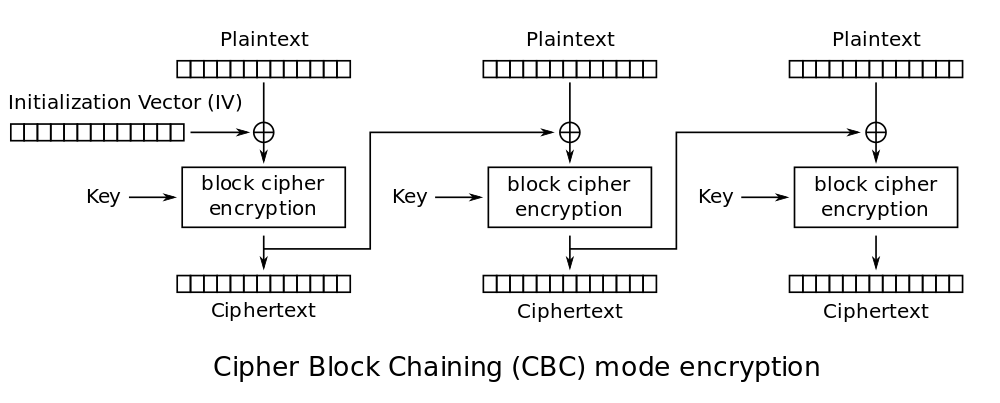
\includegraphics[width=1\textwidth, height=1\textheight, keepaspectratio]{./images/aes_modes/cbc.png} % mettere 1 e 1?
	\caption{CBC}
	\label{fig:cbc}
\end{figure}

%TODO: Ricapitolando le fasi che si evincono dallo shema, qui sopra:

\begin{itemize}
	\item \textsf{\small Collega ("Incatena" da \emph{Chaining}) tutti i blocchi.}
	\item \textsf{\small L'IV (\emph{\textbf{I}nitialization \textbf{V}ector}) è usato per modificare il testo in chiaro.}
	\item \textsf{\small Viene eseguito lo XOR tra il blocco cifrato precedente e il blocco col testo in chiaro corrente.}
	\item \textsf{\small Risolve il problema dei blocchi di testo in chiaro uguali vengano cifrati allo stesso modo. (problema presente in ECB)}
	\item \textsf{\small Modificando un bit di un blocco di testo in chiaro, modifica di conseguenza tutti gli altri blocchi cifrati a seguire.}
\end{itemize}

%TODO: Aggiungere immagine/schema della decifrazione?

%TODO: Sono possibili degli attacchi su ECB, se l'attaccante modifica ogni secondo blocco in chiaro se è a conoscenza dell'intero testo in chiaro.

%TODO: Questa modalità è sicura come uno schema probabilistico e la confidenzialità non viene raggiunta se l'IV è un nonce semplice. %TODO: forse approfondire cos'è un nonce semplice

\subsubsection{CFB | Cipher Feedback}

%TODO: CFB è molto simile a CBC, ma al posto di essere un cifrario a blocchi, è un cifrario a stream, \emph{stream cipher}, ovvero un cifrario che prende una chiave e un algoritmo e lo applica allo stream (un bit alla volta), a ogni singolo bit (bit a bit) e non a blocchi di bits.

\textsf{\small }

\begin{figure}[H]
	\centering
	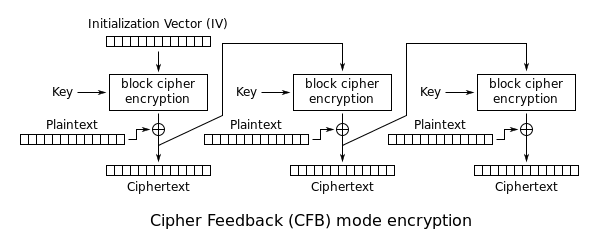
\includegraphics[width=1\textwidth, height=1\textheight, keepaspectratio]{./images/aes_modes/cfb.png} % mettere 1 e 1?
	\caption{CFB}
	\label{fig:cfb}
\end{figure}

%TODO: Ricapitolando lo schema presente qui sopra:

\begin{itemize}
	\item \textsf{\small Lega tutti i blocchi (proprio come CBC).}
	\item \textsf{\small Genera dei bytes casuali, un flusso usando il cifrario che viene poi successivamente XOR col blocco di testo in chiaro.}
	\item \textsf{\small Trasforma il cifrario a blocchi in uno stream cipher (cifrario a flusso).}
\end{itemize}

%TODO: Aggiungere immagine/schema della decifrazione?

\subsubsection{OFB | Output Feedback}

\begin{figure}[H]
	\centering
	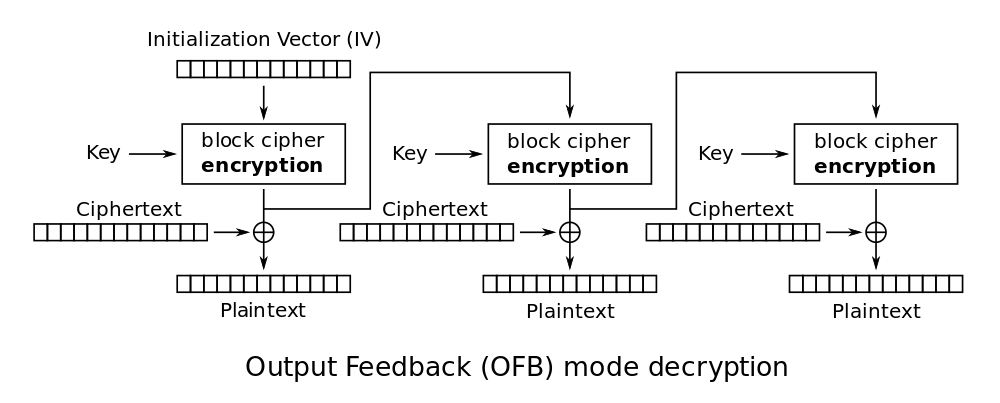
\includegraphics[width=1\textwidth, height=1\textheight, keepaspectratio]{./images/aes_modes/ofb.png} % mettere 1 e 1?
	\caption{OFB}
	\label{fig:ofb}
\end{figure}

%TODO: È anch'esso un \emph{stream cipher}, cifra l'iv (genera una serie di caratteri casuali)  e poi esegue uno XOR per ottenere il testo cifrato.
%TODO: Ogni operazione dipende da quelle precedenti.

\textsf{\small }

\textsf{\small }%TODO: Ricapitolando le operazioni dell'OFB, proprio come il CFB:

\begin{itemize}
	\item \textsf{\small Lega tutti i blocchi (proprio come CBC e CFB).}
	\item \textsf{\small Genera dei bytes casuali, un flusso usando il cifrario che viene poi successivamente XOR col blocco di testo in chiaro.}
	\item \textsf{\small Trasforma il cifrario a blocchi in uno stream cipher (cifrario a flusso).}
\end{itemize}

\textsf{\small L'unica differenza con CFB è che al posto di utilizzare il testo cifrato nei blocchi successivi, utilizza l'output dei bytes casuali generati dal cifrario attraverso la chiave e l'IV per il blocco successivo.}

\subsubsection{CTR | Counter Mode}

%TODO: La Counter Mode o CM (\emph{integer counter mode}) o SIC (\emph{segmented integer counter}) usufruisce di un counter (contatore), ovvero di una funzione che genera sequenze irripetibili (nel tempo), al posto di utilizzare un IV.
%TODO: Il più semplice contatore è il (banale/banalissimo) incrementa di 1.
%TODO: Questa modalità può essere parallelizzata.

\textsf{\small }

\begin{figure}[H]
	\centering
	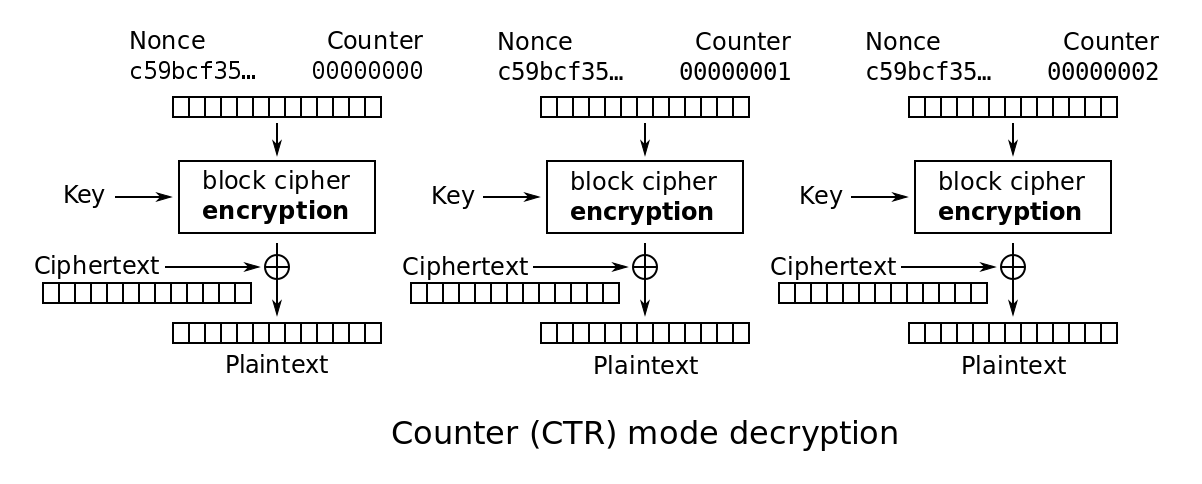
\includegraphics[width=1\textwidth, height=1\textheight, keepaspectratio]{./images/aes_modes/ctr.png}
	\caption{CTR}
	\label{fig:ctr}
\end{figure}

\subsubsection{XTS | AES-XTS (XEX) Tweakable Block Cipher}

%TODO: Questa modalità è utilizzata per cifrare/decifrare i dischi rigidi (hard-disk), quindi la cifratura verrà operata sui segmenti da 512 bytes(, ovvero 32 blocchi di AES-128,) e i rispettivi settori (del disco).

%TODO: Questa modalità esegue/è composta/compie/effettua le seguenti operazioni:

%TODO: itemize?
%TODO: Dati/Definiti: Due chiavi K1, K2 (se utilizziamo AES-128). Blocco di input, P, numero settore, \emph{i} e un numero del blocco, \emph{j}, creiamo/definiamo il tweak", \emph{X}, nel seguente modo:

%TODO: $X = E_{K_2}(i) \otimes 2^j$ 
%TODO: (\otimes è il prodotto tensoriale (nel finite field)). Da includere nel capitolo della matematica?

%TODO: Di conseguenza, il testo cifrato C è definito così:
%TODO: $C = P \oplus X$
%TODO: ovvero testo cifrato = blocco di input XORato con il tweak.
%TODO: $C = E_{K_1}(C) \oplus X$

%TODO: Per poter decriptare, invece, eseguiamo: 
%TODO: $X = E_{K_2} (i) \otimes 2^j$

%TODO: il testo in chiaro, per ogni blocco, è 
%TODO: $P = C \oplus X$
%TODO: $P = E^{-1}_{K_1} (P) \oplus X$

%TODO: In questo modo, il tweak fa da IV.

\textsf{\small }

\begin{figure}[H]
	\centering
	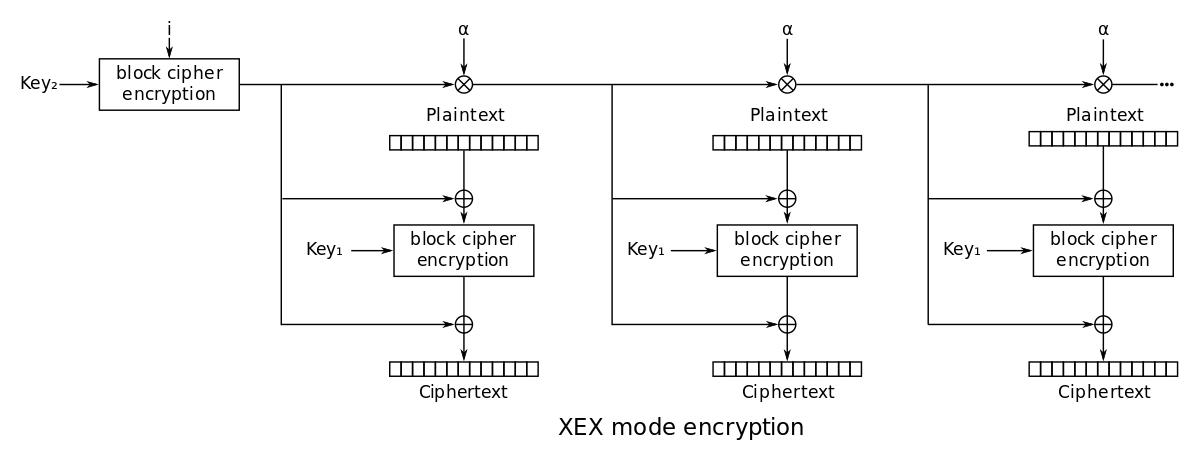
\includegraphics[width=1\textwidth, height=1\textheight, keepaspectratio]{./images/aes_modes/xex.png}
	\caption{XEX}
	\label{fig:xex}
\end{figure}

%TODO: subsection Block cipher modes, encryption but not message integrity
%TODO: subsection ECB | Electronic Code Book
%TODO: subsection Cipher Block Chain | CBC
%TODO: subsection CFB | Cipher Feedback
%TODO: subsection OCB | Offset Codebook (questo va nella subsection MACS)
%TODO: subsection CTR | Counter Mode
%TODO: subsection XTS | AES-XTS (XEX) Tweakable Blk Cipher 

%TODO: subsection EAX | encrypt-then-authenticate-then-translate. metterlo o no?

\subsection{MACS | Message Authentication Codes}

%TODO: I MACS permettono di verificare l'integrità del messaggio per potersi assicurare che non sia stato manomesso/alterato da parti esterne e che il messaggio arrivi/giunga integro/intero ai destinatari originali.

%TODO: Quindi, i MACS producono/formano una tipologia di firma digitale dove tutte le parti considerate/in considerazione possono verificare che i dati ricevuti siano validi.

%TODO: Questo grazie a un meccanismo a 3 componenti:
%TODO: itemize/enumerate
%TODO: 1. Chiave segreta: chiave segreta condivisa dalle parti.
%TODO: 2. MAC Signing Algorithm: (ci) si avvale della chiave e del messaggio per creare/generare/produrre un tag (\emph{authentication tag} che permette(, per l'appunto,) di verificare che i dati siano integri e non manomessi/truccati)
%TODO: 3.MAC Validation Algorithm: prende in input la chiave, il messaggio, il tag e restituisce in output la validità del tag, ovvero se è il messaggio è stato modificato/violato o no.

\textsf{\small }

\begin{figure}[H]
	\centering
	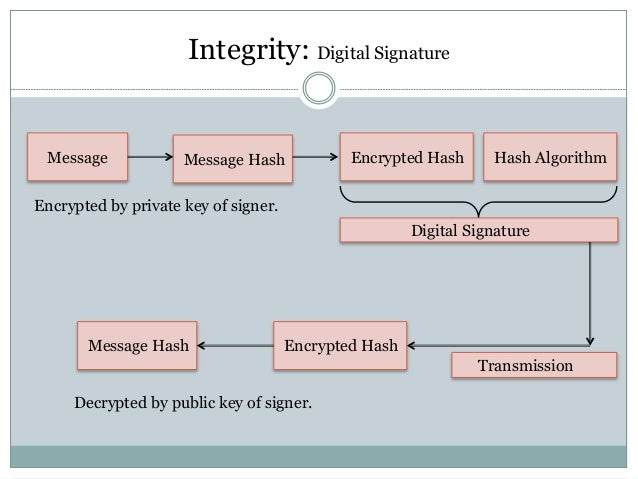
\includegraphics[width=.9\textwidth, height=.9\textheight, keepaspectratio]{./images/aes_modes/encryption-integrity-and-nonrepudiation.png}
	\caption{Integrità e non ripudio}
	\label{fig:encryption-integrity-and-nonrepudiation}
\end{figure}

\subsubsection{ALG1-6}

%TODO: È una collezione di MACs basati su CBC-MAC, di cui alcuni sicuri come il VIL PRF, FIL PRF altri non ne abbiamo certezza.

\textsf{\small }

\subsubsection{CMAC | Cipher-based Message Authentication Code}

%TODO: CMAC è una modalità basata su CBC-MAC. Questa crea un messaggio di autenticazione (MAC) utilizzando un cifrario a blocchi e una chiave segreta. 

\textsf{\small }

\begin{figure}[H]
	\centering
	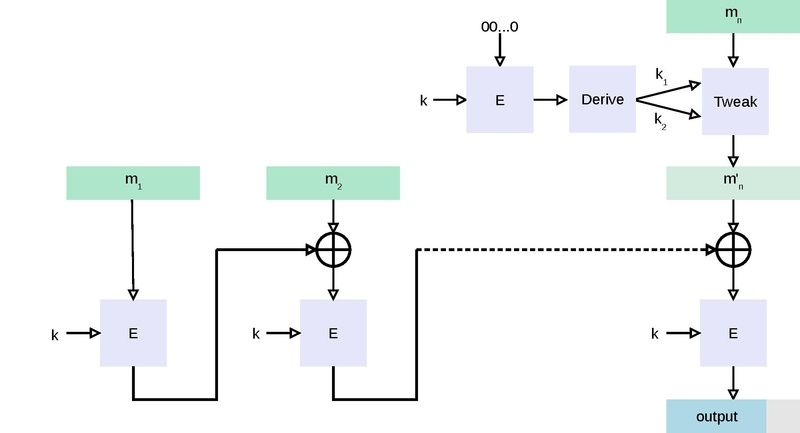
\includegraphics[width=.9\textwidth, height=.9\textheight, keepaspectratio]{./images/aes_modes/CMAC_-_Cipher-based_Message_Authentication_Code}
	\caption{CMAC}
	\label{fig:cmac}
\end{figure}

\subsubsection{HMAC | Keyed-hash Message Authentication Code}

%TODO: HMAC è una modalità che permette di autenticare gli emittenti del messaggio attraverso autenticazione basata su algoritmi di hashing, come: MD5, SHA-1, SHA-256 (SHA-2) e SHA-3.

%TODO: La sicurezza di questa modalità è stata provata.

\textsf{\small }

\subsubsection{GMAC | Galois Message Authentication Code}

%TODO: Questa modalità è una specializzazione della modalità \textbf{GCM} (\emph{\textbf{G}alois/\textbf{C}ounter \textbf{M}ode}). Viene utilizzata per l'autenticazione.

\textsf{\small }

\begin{figure}[H]
	\centering
	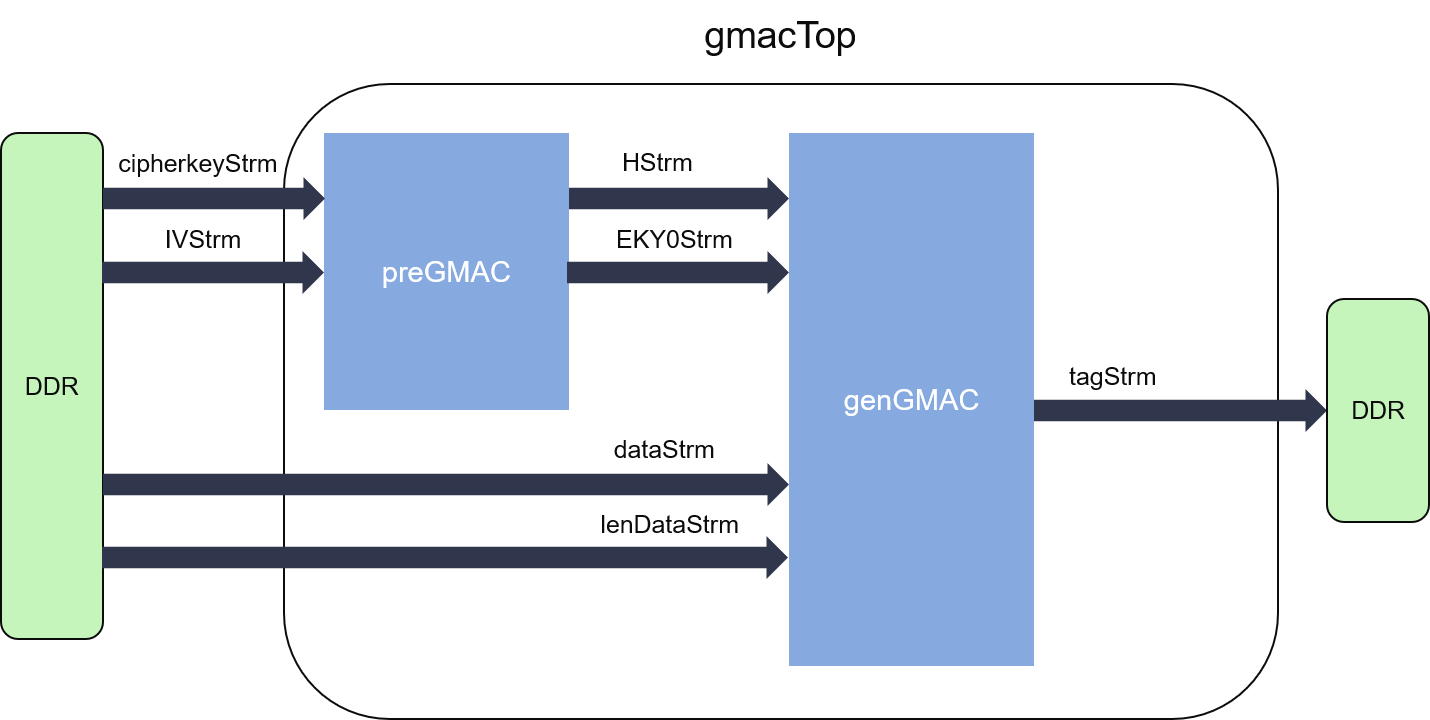
\includegraphics[width=.9\textwidth, height=.9\textheight, keepaspectratio]{./images/aes_modes/internal_structure_of_gmac} %TODO: gcm
	\caption{GMAC}
	\label{fig:gmac}
\end{figure}

\subsubsection{CBC-MAC}

%TODO: CBC-MAC combina la modalità CBC (Cipher Block Chaning) assieme al MAC per l'autenticazione dei mittenti del messaggio.

\textsf{\small }

\begin{figure}[H]
	\centering
	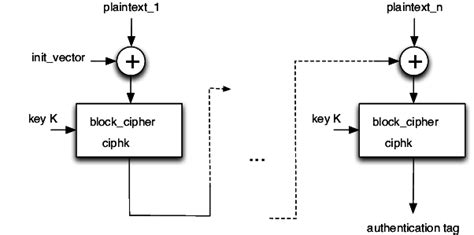
\includegraphics[width=.9\textwidth, height=.9\textheight, keepaspectratio]{./images/aes_modes/cbc-mac}
	\caption{CBC-MAC}
	\label{fig:cbc-mac}
\end{figure}

%TODO: subsection ALG1-6, CMAC (Cipher-based Message Authentication Code), HMAC (keyed-hash message authentication code o hash-based message authentication code), GMAC (Galois Message Authentication Code), CBC-MAC (CBC-MAC qui o sopra?)

\subsection{AEAD | Authenticated Encryption with Associated Data}

%TODO: AEAD è un modello di cifratura che assicura sia la riservatezza del messaggio sia la sua autenticazione.

\textsf{\small }

\subsubsection{OCB | Offset Codebook} %TODO: section MACS? AEAD

%TODO: Aggiungere qualcos'altro su questa modalità.

%TODO: Questa modalità è stata ideata da Phillip Rogaway con l'assistenza di Mihir Bellare, John Black e Ted Krovetz, basata sull'IAPM (\emph{\textbf{I}ntegrity-\textbf{A}ware \textbf{P}arallelizeable \textbf{M}ode}) che permette di parallelizzare la modalità.

%TODO: Sono presenti tre versioni di OCB: OCB1, OCB2 e OCB3.

%TODO: OCB, rispetto alle altre modalità, è molto più veloce.  

%TODO: Erano presenti due brevetti su questa modalità che ne impedivano l'esteso utilizzo [la diffusione], ma dal 2021 questi sono stati abbandonati.

\textsf{\small }

\subsubsection{CCM | Counter con CBC-MAC}

%TODO: CCM è un AEAD basato su Nonce che combina le modalità CTR e CBC-MAC i cui blocchi devono essere composti da 128 bits.

\textsf{\small }

\subsubsection{GCM | Galois Counter Mode}

%TODO: È un AEAD basato su Nonce che combina le modalità CTR per l'operazione di cifratura e il campo di Galois (Galois Field) GF(2^{128}) per l'autenticazione.

%TODO: Può essere usato come Nonce-MAC, in quel caso viene denominato \textbf{GMAC}.

\textsf{\small }

\begin{figure}[H]
	\centering
	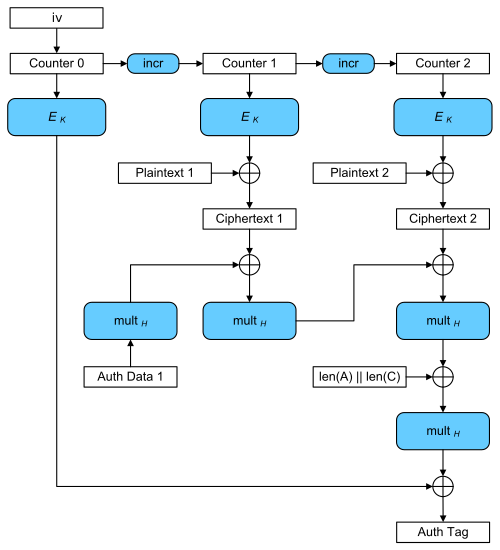
\includegraphics[width=.9\textwidth, height=.9\textheight, keepaspectratio]{./images/aes_modes/GCM-Galois_Counter_Mode_with_IV} 
	\caption{GCM}
	\label{fig:gcm}
\end{figure}

%TODO: section/subsection Authenticated Encryption (AEAD (Authenticated Encryption with Associated Data))
%TODO: CCM | Cipher Block Chaining e GCM | Galois Counter Mode